\documentclass[]{article}

%imports
\usepackage{amsmath}
\usepackage{amsthm}
\usepackage{amssymb}
\usepackage{tikz-cd}
\usepackage{quiver}
\usepackage{array}
\usepackage[all,cmtip]{xy}



\usepackage{hyperref}
\usepackage{cleveref}


\usepackage[style=alphabetic]{biblatex}

%references
\addbibresource{ref.bib}
%\bibliography{ref.bib}

%newtheorems
\theoremstyle{definition}
\newtheorem{definition}{Definition}[section]

\newtheorem{theorem}{Theorem}[section]
\newtheorem{corollary}{Corollary}[section]
\newtheorem{lemma}{Lemma}[section]
\newtheorem{proposition}{Proposition}[section]
\newtheorem{example}{Example}[section]
\newtheorem{question}{Question}

%commands
\newcommand{\mo}{\ensuremath{\text{mod }}}
\newcommand{\Hom}{\ensuremath{\text{Hom}}}
\newcommand{\tu}{\ensuremath{\tau}}
\newcommand{\Fac}{\ensuremath{\text{Fac }}}

\newcommand{\spmat}[1]{%
	\begin{bmatrix}#1\end{bmatrix}%
}




%opening
\title{Computing \tu-rigid modules}
\author{Håvard Utne Terland}

\begin{document}

\maketitle

\begin{abstract}

\end{abstract}

\newpage
\section*{Acknowledgments}
I want to thank my main advisor, Prof. Aslak Buan, for guiding me through the field representation theory, from Auslander-Reiten theory to $\tau$-tilting theory. My co-advisor Prof. Øyvind Solberg has also been of great help. In particular, I am grateful for fruitful conversations on computational aspects of representation theory and for helping me through basic ring theory during my first semester at NTNU. It is no exaggeration that I owe almost all of my intuition on module theory to these meetings with Øyvind and his detailed notes on non-commutative ring theory.
I also want to thank Dr. Eric Hanson for very constructive feedback during the $\tau$-tilting theory seminars the spring of 2021: No person has ever supplied counterexamples to overambitious claims I've made faster than Eric. I would also like to thank the algebra group at NTNU as a whole, for welcoming me to the institute as a PhD candidate on the integrated PhD program.

Outside the algebra group, I want to thank my friends in Trondheim, especially my friends from Skansegata that I lived with while writing this thesis; Andreas Gjerde, Henrik Midtun, Halvor Veiby, Marius Jünger and Vegard Strand. 



\newpage
\section{Introduction}
Representation theory of algebras may be understood as understanding the ways a finite set of linear transformations may act together on vector spaces given some constraints. This may formulated using the language of module theory, where systems of linear transformations corresponds to modules over a finite dimensional algebra derived from the class of systems of linear transformations one is studying. To be more precise, this class of systems is given as a quiver, and the constraints are given as an ideal of the path algebra over the quiver.


In these terms, representation theory of algebras then seeks to classify modules over finite dimensional algebras. For special classes of algebras, much progress has been made in this regard. However, the majority of algebras are too complicated for a proper classification of modules to be made.

To give an example, we may consider the quiver below. A representation of this quiver is simply a linear transformation from one finite dimensional vector space to some other finite dimensional vector space.
% https://q.uiver.app/?q=WzAsMixbMCwwLCJcXGJ1bGxldCJdLFsxLDAsIlxcYnVsbGV0Il0sWzAsMV1d
\[\begin{tikzcd}
	1 & 2
	\arrow[from=1-1, to=1-2]
\end{tikzcd}\]

A representation of the above is in other words given by an arbitrary $n \times m$ matrix, over the field one wishes to work over. When dealing with a single linear transformation, classical linear algebra is sufficient, and computing the rank, nullity and corank of the matrix gives you everything we need to understand the transformation (corank for an $n \times m$ matrix is $m$ minus the rank of the matrix). Thus, there is no surprise that there are three indecomposable representations of this quiver, as seen in the figure below. Thus a matrix $M$ corresponds to some number of copies of the representations $M_1,M_2$ and $M_3$. These numbers are exactly the rank, nullity and corank of $M$, respectively.

% https://q.uiver.app/?q=WzAsNixbMCwyLCJcXGJ1bGxldCJdLFsxLDIsIlxcYnVsbGV0Il0sWzAsMSwiXFxidWxsZXQiXSxbMSwxLCJcXGJ1bGxldCJdLFswLDAsIlxcYnVsbGV0Il0sWzEsMCwiXFxidWxsZXQiXSxbMCwxXSxbMiwzXSxbNCw1XV0=
\begin{figure}[h]
	\[\begin{tikzcd}
		M_1: k & k \\
		M_2: k & 0 \\
		M_3: 0 & k
		\arrow[from=3-1, to=3-2,"0"]
		\arrow[from=2-1, to=2-2,"0"]
		\arrow[from=1-1, to=1-2,"1"]
	\end{tikzcd}\]
\caption{The three indecomposable representations of the quiver with one arrow.}

\end{figure}


In this thesis, we focus not on understanding all modules, but instead focus on computing and classifying \tu-rigid modules over as general algebras as our techniques let us. The reasons for studying \tu-rigid modules come from attempt to generalize tilting theory, in particular from the perspective of mutations. Mutations give a combinatorial tool one can employ to understand \tu-tilting modules, similar to the techniques stemming from using Auslander-Reiten quivers to compute module categories. However, we may understand mutation for algebras where we cannot compute the whole AR-quiver. In this sense, \tu-tilting theory offers a new toolbox in the representation theory of algebras.




\section{Preliminaries}
Here we collect some of the necessary prerequisites for reading this thesis, in all majority results and facts not found in \cite{auslander_reiten_smalo_1995} and \cite{assem_skowronski_simson_2006} which we refer two as general references on the representation of finite dimensional algebras.

\subsection{Notation and setting}
We closely follow the notation of \cite{assem_skowronski_simson_2006}. An algebra $A$ will always refer to a finite dimensional algebra over a field $k$, which need not be algebraically closed. All algebras encountered in this thesis will be, unless otherwise stated, on the form $k\Gamma/I$ for some finite quiver $\Gamma$ and admissible ideal $I$. The number $n$ is, unless otherwise stated, reserved for the number of indecomposable projective summands of $A$. By $\mo A$ we denote the category of finite dimensional left $A$-modules (in contrast to \cite{assem_skowronski_simson_2006}, who employ right modules). We implicitly identify $A$-modules to representations of its quiver with relations. We denote by $D$ the duality on modules, and by $\text{Tr}$ the transpose. The Auslander-Reiten translate $D\text{Tr}$ is denoted $\tau$.

A module $M$ is called basic if no two nonzero summands are equal, that is $M \cong A \oplus X \oplus X$ implies $X = 0$. We denote by $|M|$ the number of indecomposable summands of $M$. 

We denote by $hom_A(M,N)$ the dimension of the $k$-vector space $\text{Hom}_A(M,N)$.

\subsection{Approximations}
Approximations are used frequently in the representation theory of algebras. In particular, they are very often used in \tu-tilting theory.

\begin{definition}
	Let $\mathcal{C}$ be a subcategory of $\text{mod} A$.  Let $M$ be an $A$-module, and $X \in \mathcal{C}$. A map $f:X \to M$ is called a \textit{right $\mathcal{C}$-approximation} of $M$ if it is the case that for any $Y \in \mathcal{C}$ and map $g:Y \to M$, there is a map $h:Y \to X$ such that $g = f \circ h$. 
	
	Let $M$ be an $A$-module, and $X \in \mathcal{C}$. A map $f:M \to X$ is called a \textit{left $\mathcal{C}$-approximation} of $M$ if it is the case that for any $Y \in \mathcal{C}$ and map $g:M \to Y$, there is a map $h:X \to Y$ such that $g = h \circ f$. 
	
	A left (right) approximation which is also left (right) minimal as a map is called a minimal left (right) approximation.
	
	If $\mathcal{C} = \text{add } M$ for a module $M$, we shorten $\text{add }M$-approximation to $M$-approximation.
\end{definition}


We say that such a subcategory $\mathcal{C}$ is \textit{contravariantly finite} (resp. \textit{covariantly finite}) if every $A$-module $M$ has a right (resp. left) $\mathcal{C}$-approximation. If $\mathcal{C}$ is both contravariantly and covariantly finite, we call it \textit{functorially finite}.


\begin{example}
	Let $M,N$ be modules in $\text{mod } A$. We may always find a left $M$-approximation of $N$ as follows. $\text{Hom}(N,M)$ is finite dimensional as a $k$-vector space, so pick a basis $F = (f_1,f_2,\dots,f_i)$. Then we have a map $f:N \to \bigoplus_{j= 1}^i M$ given by $f = \begin{bmatrix}
	f_1 \\ \vdots \\ f_i
	\end{bmatrix}$. Given any map $g_r:N \to \bigoplus_{j = 1}^k M_j$ where $M_j$ is a summand of $M$, this map will naturally factor through a map $g:N \to \bigoplus_{j = 1}^k M$, which we may describe as $g = [g_1,g_2,\dots,g_k]$. Since $F$ is a basis for $\text{Hom}(M,N)$, we may write \[g = [a_{1,1}f_1 + \dots + a_{1,i}f_i,\dots,a_{k,1}f_1 + \dots + a_{k,i}f_i]\]
	
	Interpreting $c \in k$ as a map $M \to M$ given by $c \cdot1$ where $1$ is the identity map, we can write $g$ as the composition
	\[g = \begin{bmatrix}
	a_{1,1} & \dots & a_{1,i} \\
	\vdots & \dots & \vdots \\
	a_{k,1} & \dots & a_{k,i}
	\end{bmatrix} \times \begin{bmatrix}
	f_1 \\ \vdots \\ f_i
	\end{bmatrix}
	\]
	
	and thus $g_r$ also factors through as wanted.
\end{example}

We now give an example of a non-trivial, non-minimal left approximation.

\begin{example}
	Let $A$ be the algebra defined by the quiver
	\[
	\begin{tikzcd}
	1 \arrow[r,bend left,"\alpha"] & 2 \arrow[l,bend left,"\beta"]  \\
	\end{tikzcd}
	\]
	
	modulo the relations $r^4 = 0$. Then $\text{Hom}(P(1),P(2))$ has dimension $2$, with maps $f_1(x) = x \beta$ and $f_2(x) =  x\beta\alpha\beta$. Clearly, $f_2 = (\beta\alpha) \circ f_1$. 
	
	Using the construction in the above example, the map $f = \begin{bmatrix} \beta \\ \beta\alpha\beta \end{bmatrix}$ is a left $P(2)$-approximation of $P(1)$. It is not left minimal, however. To see this, consider the endomorphism on $P(2) \oplus P(2)$ given by \[\phi = \begin{bmatrix} 1 & 0 \\ \alpha\beta & 0\end{bmatrix}\]
	
	Then $\phi \circ f = f$, but $\phi$ is not an isomorphism. 
	
	$f_1$ alone, however, is a minimal left approximation.
\end{example}


\section{Tau-tilting theory}
$\tau$-tilting theory was introduced in \cite{tau} as a possible generalization of tilting theory, which has had tremendous impact on the field of representation theory of finite dimensional algebras as a whole. Although first introduced in \cite{tau}, some of the main results of $\tau$-tilting theory stem from (cite smalø). We here recall some important definitions and results from $\tau$-tilting theory. Also, we note that there are other approaches to defining \tu-rigid pairs which are fruitful in other contexts. To make these introductory sections both concise and self-contained, we will not dwell on these alternative approaches to the theory here.  When we need different but equivalent definitions in later sections, references to the literature will be made.

We start by discussing $\tau$-rigid modules, which may be considered the building blocks of $\tau$-tilting theory. 


\begin{definition}
	A module $M$ in $\mo A$ is called $\tau$-rigid if $\Hom(M,\tau M) = 0$.
\end{definition}

First note that the Auslander-Reiten formula gives that \tu-rigid objects must be exceptional objects. Note that $X,Y$ being $\tau$-rigid does not imply $X \oplus Y$ being $\tau$-rigid. In fact, studying how indecomposable $\tau$-rigid modules together form larger $\tau$-rigid modules is part of $\tau$-tilting theory.

\begin{definition}\cite[Definition 0.3]{tau}
	A pair $(M,P)$ where $M$ is basic $\tau$-rigid and $P$ basic projective such that $\Hom_A(P,M) = 0$ is called a  $\tau$-rigid pair.
\end{definition}

Along with this definition follows many conventions. For a  $\tau$-tilting module $T = (M,P)$, $P$ will be denote the projective part of $T$ and $M$ the module part. $T$ is called support \tu-tilting if $|M| + |P| = n$, and almost complete support \tu-tilting if $|M| + |P| = n - 1$. A support \tu-tilting pair with no non-zero projective part may also be denoted a \tu-tilting module. 

For $T_1,T_2$ both \tu-rigid pairs, we consider $T_1$ a summand of $T_2$ is both the module part and the projective part of $T_1$ is a summand of the module part and the projective part of $T_2$ respectively.

\begin{example}
	Since $\tu P = 0$ for any projective module $P$, any projective module is \tu-rigid. As a consequence, $A = \oplus_{i = 1}^n P(i)$ is a \tu-tilting module.	
\end{example}

\begin{example}
	For an hereditary algebra $A$, partial tillting modules coincide with \tu-rigid modules. For $M$ partial tilting, $0 = Ext^1_A(M,M) \cong \Hom_A(M,\tu M)$, where the first equality follows from the definition of tilting-modules and the second equality follows from the Auslander-Reiten formula in the hereditary case.
\end{example}

\subsection{Torsion classes induced by support \tu-modules}
Given a support \tu-tilting pair $(M,P)$, we may consider the modules generated by $M$, $\Fac M$. As in classical tilting theory, this is a torsion class, and we have the following very important result.

\begin{theorem}\cite[Theorem 2.7]{tau}\cite{auslandersmalo81}
	There is a bijection between the set of functorially finite torsion pairs, denoted $\text{f-tors} A$ and support \tu-tilting modules, denoted $\text{s}\tu\text{-tilt} A$, given by sending a support \tu-tilting pair $(M,P)$ to $(\Fac M,M^\perp)$.
\end{theorem}

We order the objects in $\text{f-tors} A$ by inclusion on the torsion classes. Thus $(X_1,Y_1) > (X_2,Y_2)$ if $X_2 \subseteq X_1$. This induces an ordering on $\text{s}\tu A$. We denote by $Q(\text{f-tors} A)$ the Hasse-quiver of the above defined ordering on $\text{f-tors} A$.

\subsection{Mutation}
An essential property of support \tu-tilting modules is that one can \textit{mutate} at each summand. More precisely, one has the following.

\begin{theorem}
	For a almost complete support $\tau$-tilting pair $(M,P)$, there exists exactly two distinct support \tu-tilting pairs $(M_0,P_0)$ and $(M_1,P_1)$.
\end{theorem}

In the above theorem, $(M_0,P_0)$ and $(M_1,P_1)$ are said to be mutations of each other, and we may write $M_1 = \mu_X(M_0)$ where $X$ is the indecomposable summand of $M_0$ that we must replace to get $M_1$; formally, we require $M_0 = X \oplus M$ or $P_0 = X \oplus P$. In this case, we \textit{mutate} at $X$.

\begin{proposition}\cite[Definition-Proposition 2.28]{tau}
	Let $T_1$ and $T_2$ be support \tu-tilting modules which are mutations of each other. Then either $T_1 < T_2$ or $T_ 2 < T_1$. In the first case, we consider $T_2$ a right-mutation of $T_1$ and in the second case we consider $T_2$ a left-mutation of $T_1$. Note that if $T_2$ is a left-mutation of $T_1$, $T_1$ is a right-mutation of $T_2$ and vice versa.
\end{proposition}

\subsection{Mutation quivers}
We use mutation of support \tu-tilting modules to define a quiver storing information about these objects.

\begin{definition}
	The support $\tau$-tilting quiver $Q(\text{s\tu-tilt} A)$ has a vertex for each support \tu-tilting module and an arrow $T_1 \to T_2$ if $T_2$ is a left mutation of $T_1$. 
\end{definition}

In the rest of this subsection, we give examples of mutation quivers and discuss some elementary facts about them.


It turns out that mutation of support \tu-tilting module is compatible with the ordering induced by the set of functorially finite torsion classes.
\begin{proposition}
	$Q(\text{s\tu-tilt} A)$ is isomorphic to $Q(\text{f-tors} A)$.
\end{proposition}

\begin{proof}
	We have an isomorphism between the vertex sets of the two quivers. It is enough to prove that there is an arrow $(T_1,P_1) \to (T_2,P_2)$ if and only if there is an arrow $(\Fac T_1,T_1^\perp) \to (\Fac T_2,T_2^\perp)$.
	
	If there is an arrow $(\Fac T_1,T_1^\perp) \to (\Fac T_2,T_2^\perp)$, we have $\Fac T_2 \subset \Fac T_1$ and no functorially finite torsion class $T \neq T_1,T_2$ such that $\Fac T_2 \subset T \subset \Fac T_1$. By \cite[Theorem 2.33]{tau}, this implies that $(T_2,P_2)$ is a left mutation of $(T_1,P_1)$ and thus there is an arrow $(T_1,P_1) \to (T_2,P_2)$ in $Q(\text{s\tu-tilt} A)$.
	
	By \cite[Theorem 2.33]{tau}, a symmetrical argument proves the other direction.	
\end{proof}

\begin{example}
	As $\Fac A=\text{mod } A$, the support \tu-tilting module $(A,0)$ is the largest element in $Q(\text{f-tors} A)$, and any mutation $\mu_X(A)$ must be a left-mutation.
\end{example}

\begin{example}
	Let $A$ be the path algebra of the disconnected quiver with two points.
	
	\[
	\begin{tikzcd}
	\bullet & \bullet   \\
	\end{tikzcd}
	\]
Then $Q(s\tau\text{-tilt} A)$ may easily be computed to be 

% https://q.uiver.app/?q=WzAsNCxbMSwwLCIoUCgxKVxcb3BsdXMgUCgyKSwwKSJdLFsxLDIsIigwLFAoMSlcXG9wbHVzIFAoMikpIl0sWzIsMSwiKFAoMSksUCgyKSkiXSxbMCwxLCIoUCgyKSxQKDEpKSJdLFswLDNdLFszLDFdLFswLDJdLFsyLDFdXQ==
\[\begin{tikzcd}
& {(P(1)\oplus P(2),0)} \\
{(P(2),P(1))} && {(P(1),P(2))} \\
& {(0,P(1)\oplus P(2))}
\arrow[from=1-2, to=2-1]
\arrow[from=2-1, to=3-2]
\arrow[from=1-2, to=2-3]
\arrow[from=2-3, to=3-2]
\end{tikzcd}\]
\end{example}

We now show how the \tu-tilting theory of a disconnected algebra is determined by its components.

\begin{definition}
	Let $Q_1,Q_2$ be quivers with vertex sets $Q_1^0$, $Q_2^0$ and arrow sets $Q_1^1$, $Q_2^1$. The Cartesian product $Q = Q_1 \mathbin{\Box} Q_2$ is defined as the quiver with vertex set $Q_1^0 \times Q_2^0$ and edges on the form $(x_1,y_1) \to (x_2,y_2)$ such that either $x_1 = x_2$ and $y_1 \to y_2$ is an edge in $Q_2^1$, or $y_1 = y_2$ and $x_1 \to x_2$ is an edge in $Q_1^2$.
	\end{definition}

\begin{lemma}
	Let $\Lambda = A \times B$ be a disconnected algebra. Then $Q(s\tu\text{-tilt} \Lambda) \cong Q(s\tu\text{-tilt} A)\mathbin{\Box}Q(s\tu\text{-tilt} B)$ as quivers.
	\end{lemma}
\begin{proof}
$(M,P) = (M_A \oplus M_B,P_A \oplus P_B)$ is support \tu-tilting over $\Lambda$ if and only if $(M_A,P_A)$ is support \tu-tilting over $A$ and $(M_B,P_B)$ is support \tu-tilting over $B$. This follows from the general fact that the module category of $\Lambda$ is the product of the module category of $A$ and the module category of $B$. More concretely, one can see that computing the Auslander-Reiten translate of $M_A$ in $A$ is essentially exactly the same operation as computing it in $\Lambda$, and this is the only nontrivial observation needed.
	
This allows us to compute $Q(s\tu\text{-tilt} \Lambda)$ as the Cartesian product of $Q(s\tu\text{-tilt} A)$ and $Q(s\tu\text{-tilt} B)$. To see this, let $(X,Y)$ be a point in $Q(s\tu\text{-tilt} A) \mathbin{\Box} Q(s\tu\text{-tilt} B)$ Then $X \oplus Y$ is clearly a point int $Q(s\tu\text{-tilt} \Lambda) $ and vice versa. Thus we have a natural bijection between the graphs, we need to investigate the edges. Let $(X_1,Y) \to (X_2,Y)$ be an edge in $Q(s\tu\text{-tilt} A) \mathbin{\Box} Q(s\tu\text{-tilt} B)$.  Then $(X_1 \oplus Y) \to (X_2 \oplus Y)$ is a valid mutation as only one summand has changed, thus corresponding to an edge in $Q(s\tu\text{-tilt} \Lambda)$, and similarly for edges on the form $(X,Y_1) \to (X,Y_2)$. Since all edges in $Q(s\tu\text{-tilt} A)\mathbin{\Box}Q(s\tu\text{-tilt} B)$ are on one of these forms, and clearly all edges in $Q(s\tu\text{-tilt} \Lambda)$ come from these edges, we have a quiver isomorphism.
 	
\end{proof}

One may also consider the graph-theoretical properties of $Q(\text{s\tu-tilt} A)$ by forgetting the orientation of the edges. From the properties of mutation, it follows at once that the mutation graph is $(n-1)$-regular. It may be finite or infinite. In the finite case the graph is connected\cite[Corollary 3.10]{tau}.

\subsection{g-vectors}
For an indecomposable module $M$, let $P_1 \to P_2 \to M \to 0$ be a minimal projective presentation of $M$, where $P_1 \cong \bigoplus_{i = 1}^n P(i)^{v_i}$ and $P_2 \cong \bigoplus_{i = 1}^n P(i)^{u_i}$. We may consider $(v_1,v_2,\dots,v_n)$ and $(u_1,u_2,\dots,u_n)$ to be vectors describing the building blocks of $P_1$ and $P_2$ respectively. Then we define $g^M$ to be $u - v$. 

\begin{definition}
	For a $\tau$-rigid pair $(M,P)$, its $g$-vector is defined as $g^M - g^P$. 
\end{definition}

Further, we follow \cite{schroll2020tautilting} and define $G$-matrices as follows.

\begin{definition}\cite[Definition 2.4]{schroll2020tautilting}
	For a support \tu-tilting pair $(M,P) = (M_1 \oplus \dots \oplus M_i,P_1 \oplus \dots \oplus P_j)$, we define its G-matrix $G_{(M,P)}$ to be the $n \times n$ matrix $(g^{M_1},g^{M_2},\dots,g^{M_i},-g^{P_1},\dots,-g^{P_j})$, where we consider the $g$-vectors to be column vectors.
	
\end{definition} 

An important property of $g$-vectors is that they uniquely identify $\tau$-rigid pairs\cite[Theorem 5.5]{tau}. This immediately gives a combinatorial proof that the set of indecomposable \tu-rigid objects must be countable (a fact known more generally for the set of exceptional objects up to isomorphism), as there are only countably many integer vectors of dimension $n$. 

Further, $G$-matrices of support \tu-tilting pairs are invertible. This follows immediately from \cite[Theorem 5.1]{tau}.

Another often-used fact is the following result.

\begin{theorem}\cite{auslander1985modules}[Theorem 1.4(a)]
	Let $M,N$ be modules. We have \[\langle g^M,[N]\rangle = hom_A(M,N) - hom_A(N,\tau M))\]
\end{theorem}


\subsection{Duality}
There is a duality between the \tu-tilting of $A$ and the \tu-tilting of $A^\text{op}$.

\section{Jasso reduction}
Using techniques from classical tilting theory, Gustavo Jasso\cite{jassoreduction} introduced reduction techniques, now often called Jasso reduction, for partial support \tu-tilting modules, and showed that one can relate the \tu-tilting theory of $A$ to the \tu-tilting theory of these reduced algebras.

This theory is now fundamental to \tu-tilting theory. Here we recall some important aspects of Jasso reduction, and refer to the original paper for a more detailed account.

Let $M$ be a basic \tu-rigid module with $k$ summands. The \textit{Jasso perpendicular} subcategory $J(M)$ is defined as \[J(M) = M^\perp \cap \, ^{\perp}\tau M\]

Jasso has shown that $J(M)$ is equivalent to a module category $\text{mod} \Lambda$ where $\Lambda$. We may obtain $\Lambda$ the following way. Let $B = M \oplus N$ be the Bongartz completion of $M$. Then let $\Lambda = \text{End}_A(B,B)/e_M$, where $e_M$ is the idempotent associated to the projective $\text{End}_A(B,B)$-module $\text{Hom}_A(B,M)$.


\begin{theorem}\cite[Theorem 3.15]{jassoreduction}
	Let $M$ be a basic \tu-rigid module. There is a bijection between the support \tu-tilting modules of $A$ having $M$ as a summand and the support \tu-tilting modules of the algebra with module category $C(M)$. Further, this bijection is order-preserving and respects mutation.
\end{theorem}

We may extend Jasso reduction to partial support \tu-tilting objects, not only \tu-rigid modules by the fact that that a partial support \tu-tilting object $(M,P)$ over $A$ is a \tu-rigid $A/e$-module where $e$ is the idempotent associated to $P$ \cite{tau}.

The above theorem shows that we can understand the \tu-tilting theory of module categories on the form $J(T)$ via the \tu-tilting theory of the whole module category. 

\begin{corollary}
	Let $A$ be a \tu-tilting finite algebra, and $T$ a partial support \tu-tilting module. Let $B$ be an algebra with module category $J(T)$. Then $B$ is \tu-tilting finite.
\end{corollary}

\begin{proof}
	Since we may embed the mutation quiver $Q = Q(s\tu\text{-tilt} B)$ in the finite quiver $Q(s\tu\text{-tilt} A)$, $Q$ itself must be finite.
\end{proof}


\section{The wall and chamber structure of finite dimensional algebras}
We here introduce the wall and chamber structure of a finite dimensional algebra $A$, and recall how it may be used to study the \tu-tilting theory of $A$. We closely follow the theory as developed in \cite{Br_stle_2019} and \cite{dij17}.

\subsection{Stability conditions}

We let $\langle -,-\rangle$ be the standard inner product on $\mathbb{R}^n$, i.e \[\langle (v_1,v_2,\dots,v_n),(w_1,w_2,\dots,w_n) = \sum_{i = 1}^{n}v_iw_i\]

\begin{definition}\cite{Br_stle_2019}[Definition 3.1]
	For $v \in \mathbb{R}^n$, a nonzero module $M \in \text{mod} A$ is called \textit{$v$-stable} if $\langle v,[M]\rangle = 0$ and $\langle v,[N]\rangle < 0$ for all proper submodules $N$. $M$ is called \textit{$v$-semistable} if $\langle v, [M]\rangle = 0$ and $\langle v, [N]\rangle \leq 0$ for every submodule $N$.
\end{definition}

We denote by $\mathcal{D}(M)$ the set of vectors $v \in \mathbb{R}^n$ such that $M$ is $v$-semistable. We call $\mathcal{D}(M)$ the stability space of $M$.


Stability spaces need not be linear spaces. However, they are always closed under positive scaling and induce linear spaces as their span. The \textit{walls} of the wall and chamber structure of A are defined as the stability spaces which induce linear spaces of codimension 1. We now describe the chambers.

Let $X^c$ denote the compliment of a set $X$ in a topological space, and $\overline{X}$ its closure. Let \[\mathcal{R} = (\overline{(\cup_{M \in \text{mod} A} \mathcal{D}(M))})^c\] \textit{chamber} in the wall and chamber structure of $A$ is defined to be a connected component of $\mathcal{R}$.

We now show that all walls are given by stability spaces of indecomposable modules, before demonstrating some examples.

\begin{proposition}
	$\mathcal{D}(M)$ be a wall. Then there is an indecomposable module $X$ such that $\mathcal{D}(M) = \mathcal{D}(X)$.
\end{proposition}

\begin{proof}
	If $M$ is indecomposable, we let $X = M$. If not, let $M = X\oplus N$, where $N,X \neq 0$. Let $v \in \mathcal{D}(M)$. Then $\langle v,[X]\rangle \leq 0$ and $\langle v,[M]\rangle \leq 0$. Since $\langle v,[M]\rangle = \langle v,[X]\rangle + \langle v,[N]\rangle = 0$, we see that $v \in \mathcal{D}(X)$. Since $[X] \neq 0$, $\mathcal{D}(X)$ must have co-dimension 1. This completes the proof.
\end{proof}

\begin{example}
	Let $A = A_2$. We compute its wall and chamber structure. We have three indecomposable $A$-modules, $S(1),S(2)$ and $P(1)$. Clearly $\mathcal{D}(S(1)) = \{(0,y): y \in \mathbb{R}\}$ and $\mathcal{D}(S(2)) = \{(x,0): x \in \mathbb{R}\}$. We now compute $\mathcal{D}(P(1))$. Let $(x,y) = v \in \mathcal{D}(P(1))$. We then require $\langle v,(1,1)\rangle = 0$ and $\langle v,(0,1)\rangle \leq 0$. The second condition implies that $y \leq 0$. The first condition implies that $x = -y$, and these two conditions are sufficient for $v$ to be in the stability space of $P(1)$. Thus the stability space of $P(2)$ is the ray $\{\alpha(1,-1) :  \alpha \in \mathbb{R}, \alpha \geq 0\}$. 
\end{example}


\subsection{Cones, walls and chambers induced by \tu-tilting pairs}
We now aim to recover information about the \tu-tilting theory of an algebra from its wall and chamber structure.

An important ingredient in this section is the following formula.
\begin{proposition}\cite{Br_stle_2019}[Corollary 3.10]
	Let $(M,P)$ be a \tu-rigid pair. Then
 \[\langle g^{(M,P)},[N]\rangle = hom_A(M,N) - hom_A(N,\tau M) - hom_A(P,N)\]
\end{proposition}

\begin{proof}
	By \cite{auslander1985modules}[Theorem 1.4(a)], we have $\langle g^M,[N]\rangle = hom_A(M,N) - hom_A(N,\tau M)$. Since $g^{(M,P)} = g^M - g^P$, we get
	\begin{align}
	&\langle g^{(M,P)},[N]\rangle \\
	&=\langle g^M,[N]\rangle - \langle g^P,[N]\rangle \\
	&=hom_A(M,N) - hom_A(N,\tau M) - hom_A(P,N) + hom_A(N,\tau P) \\
	&=hom_A(M,N) - hom_A(N,\tau M) - hom_A(P,N) + hom_A(N,0)\\
	&=hom_A(M,N) - hom_A(N,\tau M) -hom_A(P,N)
	\end{align}
\end{proof}

Note that the above formula implies that a diension vector $[X]$ with $X$ in $J(M,P) = J(M_1\oplus\dots\oplus M_i,P_1\oplus\dots\oplus P_j)$ will be orthogonal to $g^{(M,P)}$. Also, by additivity, $[X]$ will be orthogonal to any linear combination of the vectors $\{g^{M_1},\dots,g^{M_i},-g^{P_1},\dots,-g^{P_j}\}$. We now aim to prove a partial converse to this statement.
\begin{definition}
	Let $T = (M,P)$ be a \tu-rigid pair. Following \cite{dij17}, we define the \textit{cone} spanned by $T$, as \[C(T) = \{\sum_{i = 1}^{j} \alpha_ig^{M_i} - \sum_{i = 1}^{k}\beta_ig^{P_i} : \alpha_i,\beta_i \geq 0 \text{ for all } i\}\]
	
	The interior $C^\circ(T) \subset C(T)$ is defined by requiring all coefficients $\alpha_i,\beta_i$ to be strictly positive.
\end{definition} 

Given a vector $\alpha = (\alpha_1,\alpha_2,\dots,\alpha_n)$ with $\alpha_i \geq 0$ for all $i$, we let $\alpha(M,P)$ denote the vector $G^{(M,P)} \times \alpha$.

\begin{proposition}\cite{Br_stle_2019}[Proposition 3.13]
	For $\alpha(M,P) \in C^\circ(M,P)$, a module $N$ is $\alpha(M,P)$-semistable if and only if $N \in J(M,P)$.
\end{proposition}

Note that the simple objects in $J(M,P)$ are, by the proposition above, exactly the $\alpha(M,P)$-stable modules.

The cones $C(T)$ for support \tu-tilting modules and almost complete support \tu-tilting modules play an important role in the wall and chamber structure of an algebra. We summarize some of the most important results below.

\begin{proposition}\cite[Proposition 3.15, Corollary 3.16, Corollary 3.21]{Br_stle_2019}\label{tau-wall-chamber-result}, \cite[Theorem 3.17]{asai2020wallchamber}
	\begin{enumerate}
		\item For a support \tu-tilting object $T_1 = (M,P)$, $C^\circ(T_1)$ defines a chamber in the wall and chamber structure of $A$.
		\item For an almost complete support \tu-tilting object $T_2 = (M,P)$, $C(T_2)$ is included in a wall $\mathcal{D}(N)$ in the wall and chamber structure of $A$. The module $N$ may be computed given the two support \tu-tilting modules containing $(M,P)$.
		\item All chambers are on the form $C^\circ(T)$ for a support \tu-tilting object $T$. \cite{Br_stle_2019} show this for \tu-tilting finite algebra, while \cite{asai2020wallchamber} demonstrates this in general. 
		
	\end{enumerate}
\end{proposition}


\begin{example}
	Consider the Kronecker algebra $K_2$. Let $M$ be an indecomposable module with dimension vector $(1,1)$. Then $\mathcal{D}(M) = \{(-1,1)\}$. However, there is no \tu-rigid module with $g$-vector $(-1,1)$, as $\text{Hom}_A(P(1),P(2)) = 0$.
\end{example}


Using the third point of \cref{tau-wall-chamber-result}, we may conclude that an algebra with infinitely many walls in its wall and chamber structure will be \tu-tilting infinite. It is well known that algebras whose quivers have a double arrow are representation infinite. Here we show that they are \tu-tilting infinite as well.
\begin{proposition}
	Any algebra $A = k\Gamma/I$ where $\Gamma$ has a double arrow is \tu-tilting infinite.
\end{proposition}

\begin{proof}
	We remark that there exists shorter proofs than the one given here. We choose to give this particular proof, because it gives an elementary example of working with the walls of an algebra.
	
	We note that the proof is very much inspired by the proof of \cite[Theorem 4.14]{Br_stle_2019}. Label the vertices of $\Gamma$ such that the double arrows are from $1 \to 2$. Then any module over $K_2$ may be canonically embedded as a module of $A$, and in particular we have for any $n \geq 2$ a module $M_n$ with dimension vector $x = (n,n+1,0,\dots,0)$, such that its proper submodules have dimension vectors $(n-k,n+1-k,0,\dots,0)$ for $1 \leq k \leq n$. We investigate $D(M_n)$.
	
	Let $v = (v_1,v_2,\dots,v_n) \in D(M_n)$. We have $\langle v,x \rangle = 0$ and $\langle v,x - (k,k,0,0,\dots,0)\rangle \leq 0$ for all integers $1 \leq k \leq n$. Thus for $i > 2$, $v_i$ may be chosen freely. Also, letting $k = n$ in the second condition, we see that $v_2 \leq 0$. The first condition implies $v_1 = \frac{-(n+1)}{n}v_2$.
	
	Assume now that $y = (y_1,y_2,\dots,y_n)$ such that the two above properties hold, namely $y_2 \leq 0$ and $y_1 = \frac{-(n+1)}{n}y_2$. We then clearly have $\langle y,[M]\rangle = 0$. We now check that for all $N \subseteq M$, we have $\langle y,[N]\rangle \leq 0$. 
	
	\begin{align}
	&\langle (\frac{-(n+1)}{n}y_2,y_2), (n-k,n+1-k)\rangle \\
	=&\langle (\frac{-(n+1)}{n}y_2,y_2), (j,j+1)\rangle \\
	=& y_2((-nj-j)/n + (j+1)) \\
	=& y_2((-nj - j + nj + n)/n) \\
	=& y_2((n-j)/n)) \\
	\leq& 0\text{, since } j \leq n
	\end{align}
	
	Thus $y$ is in $D(M_n)$. Since we may chose $y_i$ for $i > 2$ freely, and any non-positive $y_2$, $D(M_n)$ generates a linear space of codimension $1$, and is thus a wall in the wall and chamber structure of $A$.
	
	Further, letting $m,n \geq 1$, it is easy to see that $D(M_n) = D(M_m)$ implies $m = n$. Thus we have identified an infinite number of walls in the wall and chamber structure of $A$, meaning that $A$ is \tu-tilting infinite.
	
\end{proof}


\subsection{Consequences for the structure of $Q(s\tu\text{-tilt})$}


This following result shows that cones of $\tau$-rigid objects intersect in a very controlled fashion.

\begin{proposition}\cite[Corollary 6.7, b)]{dij17}
	Let $T_1,T_2$ be support \tu-tilting objects. Then $C(T_1) \cap C(T_2) = C(X)$ with $X$ being the maximal \tu-rigid pair such that $X$ is a summand of $T_1$ and of $T_2$.
\end{proposition}

This result gives a tool for classifying all support \tu-tilting objects. We collect this technique as a proposition.

\begin{proposition}\cite{dij17}
	Let $A$ be an algebra.
	
	\begin{itemize}
		\item If $A$ is \tu-tilting finite, its mutation graph is connected, thus the set of support \tu-tilting modules over $A$ are exactly the ones in this component.
		\item If it is \tu-tilting infinite the mutation graph may be disconnected. Let $X$ be a set of support \tu-tilting modules such that $\cup_{T \in X} C(T)$ is dense in $\mathbb{R}^n$. Then $X$ contains all support \tu-tilting modules over $A$.
		
	\end{itemize}
\end{proposition}

\begin{proof}
	The \tu-tilting finite case is well-known. We note that the second point also holds in this case, but is not needed as connectivity of the mutation graph is sufficient to to compute all support \tu-tilting modules.
	
	Let $T = (M,P)$ be a support \tu-tilting object. Consider a point $x \in C(T)$ in the interior of $C(T)$. Since $\cup_{T \in X} C(T)$ is dense in $\mathbb{R}^n$, there is a $T_2$ in $X$ such that $C(T_2) \cap C(T)$ contains $x$. But $C(T_2)\cap C(T) = C(Y)$ for some partial suport \tu-tilting object $Y$. Since $T \neq T_2$, there is a summand $Z$ in $T = (M,P)$ not in $Y$. Writing $x$ as an element of $C(T)$, we get
	
	\[x = \sum_{i = 1}^{j} \alpha_ig^{M_i} - \sum_{i = 1}^{k}\beta_ig^{P_i}\]

	The above expression also gives a way of writing $x$ as an element of  $C(T)$, where in particular the $g^{Z}$ coordinates are $0$. Thus $x$ lies on the border of $C(T)$, giving us a contradiction.
	
\end{proof}

It is interesting to note that for tame algebras, the converse of the above theorem holds, in the sense that the closure of the union of all chambers must span $\mathbb{R}^n$, see \cite{keller2020tame}.

in \cite{dij17}, the authors use the above demonstrated criteria to classify the support \tu-tilting objects of two specific symmetric algebras. We may however easily refine the criterion using ideas from\cite{Br_stle_2019}. We collect this refined technique as a theorem, which will be used frequently in this thesis.

\begin{theorem}
	Let $A$ be an algebra. Let $W$ be the set of walls in the wall and chamber structure of $A$, and let $\overline{W}$ be its closure.
	
	Let $X$ be a set of support \tu-tilting modules whose cones hit all chambers of $A$, i.e such that \[(\cup_{T \in X} C(T))  \cup \overline{W} = \mathbb{R}^n\]  then $X$ contains all support \tu-tilting modules over $A$.
\end{theorem}

\begin{proof}
	The set of chambers $C$ in the wall and chamber structure of $A$ is defined as the connected components of $\mathbb{R}^n - \overline{W}$. If $(\cup_{T \in X} C(T))  \cup \overline{W} = \mathbb{R}^n$, then $\mathbb{R}^n - \overline{W} \subseteq (\cup_{T \in X} C(T))$. Thus every chamber $c \in C$ lies entirely inside $(\cup_{T \in X} C(T))$. Since now chambers of different support \tu-tilting objects may only intersect on their boundary, we may conclude that $c \in X$. This finishes the proof.
\end{proof}


\subsection{Wall crossing and green sequences}
We may also use the wall and chamber structure to detect the non-existence of maximal green sequences. A maximal green sequence in $Q(s\tu\text{-tilt} A)$ is a path from $(A,0)$ to $(0,A)$ using only left mutations, i.e respecting the orientation of the edges in the mutation quiver.

We will see that mutations in $Q(s\tu\text{-tilt} A)$ are closely linked to certain paths in the wall and chamber structure of $A$.

\begin{definition}%add citation
	A smooth path $\gamma:[0,1] \to \mathbb{R}^n$ is called a $\mathcal{D}$-generic path if:
	
	\begin{enumerate}
		\item Both $\gamma(0)$ and $\gamma(1)$ lie in the interior of some chamber.
		\item If $\gamma(t)$ lies in the intersection of two walls, the dimension vectors of the modules determining these walls must be scalar multiples of each other. Note that this means that $\gamma(t) \neq 0$ for all $t$.
		\item $\gamma(t) \in \mathcal{D}(M)$ implies $\langle \gamma'(t),[M]\rangle \neq 0$.
	\end{enumerate}

	Further, when $\gamma(t)$ lies in a wall $\mathcal{D}(M)$, we say that the crossing is \textit{green} if $\langle \gamma'(t),[M]\rangle > 0$ and red if $\langle \gamma'(t),[M]\rangle < 0$. A $\mathcal{D}$-generic path is then called green if all such crossings are green.
\end{definition}

In \cite[Lemma 4.2]{Br_stle_2019}, the authors construct explicitly a $\mathcal{D}$-generic path moving from the chamber of some support \tu-tilting pair $(M,P)$ to the chamber induced by a mutation of $(M,P)$, passing exactly one wall.

Inductively, they show that a sequence of left and right mutations from $(M_1,P_1)$ to $(M_2,P_2)$ induces a $\mathcal{D}$-generic path between $C^\circ(M_1,P_1)$ and $C^\circ(M_2,P_2)$ passing one wall for each mutation. The following corollary will be used later.

\begin{corollary}\label{corollary-dgeneric}
	Let $T = (M_1,P_1)$ and $T = (M_2,P_2)$ be support \tu-tilting objects over $A$.
	
	If there is no $\mathcal{D}$-generic path $\gamma$ from $C^\circ(T_1)$ and $C^\circ(T_2)$ in the wall and chamber structure of $A$ passing only finitely many walls, then $T_1$ and $T_2$ lie in different components of $Q(s\tau\text{-tilt} A)$
\end{corollary}

\begin{proof}
	This is the contra-positive of [Theorem 4.3]\cite{Br_stle_2019}.
\end{proof}

\section{Main results}
We now exploit the techniques discussed so far to determine properties of mutation quivers $Q(s\tau\text{-tilt} A)$ for various algebras $A$.


\subsection{Inheriting mutation from Kronecker algebras}
The idea of the following theorem is to use the \tu-tilting theory of the Kronecker algebra with two arrows, $K_2$, to explicitly compute mutations in a more complicated algebra.

\begin{theorem}\label{k2-reduction}
	Let $A$ be an algebra on the form $kQ/r^2$ where $Q$ is the quiver	
	\[\begin{tikzcd}
	1 
	\arrow[r,bend left,shift right = 0.5ex, "\beta"]
	\arrow[r,bend left, shift left = 2ex, "\alpha"]
	& 2 \arrow[l,bend left,shift right = 0.5ex,"\gamma"]
	\arrow[l,bend left,shift left = 2ex, "\delta"]  \\
		\end{tikzcd}
	\]
	
	Then $Q(s\tau\text{-tilt } A)$ has exactly two components.
		
\end{theorem}



\begin{proof}
	A module $M$ over $A$ where either the maps induced by $\gamma$ and $\delta$, or $\alpha$ and $\beta$ are zero may naturally be considered a $K_2$-module.
	
	Then it is not difficult to see that the $g$-vector of such an $M$ as a $K_2$-module is the same as the $g$-vector of $M$ as an $A$-module, up to switching coordinates (if we demand that arrows go from vertex $1$ to $2$ in $K_2$, we need to do this swap for the case where $M$ is an $A$-module where $\alpha,\beta$ are zero).
	
	Consider the mutation of $P(1) \oplus P(2)$ at $P(1)$.
	
	\[P(1) \xrightarrow{\begin{bmatrix} \gamma \\ \delta\end{bmatrix}} P(2) \oplus P(2)\]
	
	Is a minimal right $P(2)$-approximation of $P(1)$, and its cokernel $X$ is naturally a $K_2$ module, as $\alpha X = 0$, and $\beta X= 0$. It is also $\tau$-rigid as a $K_2$ module. We thus have a \tu-tilting pair $T = (P(2),X)$ over $A$, which may naturally be considered a \tu-tilting pair over $K_2$. 
	
	This means that all iterated left mutations from $T$ are controlled by mutation in $K_2$. 
	
	A symmetrical argument shows that mutating $P(1) \oplus P(2)$ at $P(2)$ gives a \tu-tilting module whose iterated left-mutations are again dictated by mutation on $K_2$.
	
	Thus we may compute the $g$-vectors of these \tu-tilting modules, as shown in the figure.
	
	
		\begin{figure}[h]
			\begin{center}
			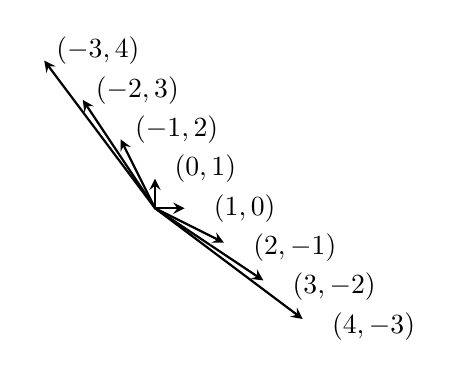
\begin{tikzpicture}[>=stealth,scale=0.5,line cap=round,
		bullet/.style={circle,inner sep=1.5pt,fill}]
		%\draw[->] (-5,0) -- (5,0) node[right]{$x$};
		%\draw[->] (0,-5) -- (0,5) node[above]{$y$};
		%\draw foreach \X in {3,6}
		%{(\X,0.1) -- ++ (0,-0.2) node[below]{$\X$}};
		%\draw foreach \Y in {2,4}
		%{(0.1,\Y) -- ++ (-0.2,0) node[left]{$\Y$}};
		\foreach \X [count=\Y] in {(1,0),(0,1),(-1,2),(-2,3),(-3,4),(2,-1),(3,-2),(4,-3)} 
		{\path  \X node(n\Y)[label=right:{$\X$}]{};
			\draw[thick,->]  (0,0) -- (n\Y);}
		\end{tikzpicture}
			\end{center}
		\caption{The $g$-vectors given by indecomposable summands of support \tu-tilting objects at most three left mutations from $(P(1) \oplus P(2),0)$ for the algebra $A$}
		\end{figure}
	
	The closure of the cones coming from the support \tu-tilting objects which are left mutations of $(P(1) \oplus P(2),0)$ clearly hit any point $(x,y) \in \mathbb{R}^2$ where $y + x \geq 0$. 
	
	By duality on support $\tu$-tilting objects, we may see that the closure of the cones coming from iterated right mutations of $(0,P(1)\oplus P(2))$ hit any point $(x,y) \in \mathbb{R}^2$ where $y + x \leq 0$. 
	
	Thus we see that every point $(x,y) \in \mathbb{R}^2$ lies in the closure of the cones coming from support \tu-tilting objects in these two components. This concludes the proof.
	
	
\end{proof}

We may generalize the theorem above slightly.
\begin{corollary}
	Let $A_{i,j}$ be the algebra on the form $kQ/r^2$ where $Q$ is on the form
	\[\begin{tikzcd}
	1
	\arrow[r, shift right = -3.5ex, draw=none, "\raisebox{+2.5ex}{\vdots}" description]
	\arrow[r,bend left,shift right = 0.5ex, "\alpha_i"]
	\arrow[r,bend left, shift left = 4ex, "\alpha_1"]
	& 2 \arrow[l, shift left = 5.0ex, draw=none, "\raisebox{+2.5ex}{\vdots}" description]
	\arrow[l,bend left,shift right = 0.5ex,"\beta_j"]
	\arrow[l,bend left,shift left = 4.0ex, "\beta_1"]  \\
	\end{tikzcd}
	\]
	
	Then $Q(s\tu\text{-tilt} A_{i,j})$ has exactly two connected components for all $i,j \geq 2$.
	
\end{corollary}

\begin{proof}
Entirely equivalent to the case where $i = 2 = j$, we will still have that left mutations of $P(1) \oplus P(2)$  behave as if they were left mutations appearing in the Kronecker algebra case.

	\begin{figure}[h]
	\begin{center}
		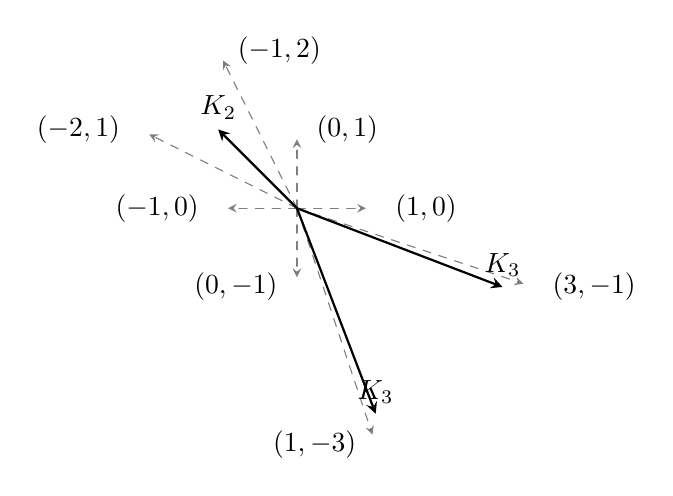
\begin{tikzpicture}[>=stealth,scale=1,line cap=round,
		bullet/.style={circle,inner sep=1.5pt,fill}]
		%\draw[->] (-5,0) -- (5,0) node[right]{$x$};
		\draw[thick,->] (0,0) -- (2.61,-1) node[above]{$K_3$};
		\draw[thick,->] (0,0) -- (1,-2.61) node[above]{$K_3$};
		\draw[thick,->] (0,0) -- (-1,1) node[above]{$K_2$};
		%\draw foreach \X in {3,6}
		%{(\X,0.1) -- ++ (0,-0.2) node[below]{$\X$}};
		%\draw foreach \Y in {2,4}
		%{(0.1,\Y) -- ++ (-0.2,0) node[left]{$\Y$}};
		\foreach \X [count=\Y] in {(1,0),(0,1),(-1,2),(3,-1)} 
		{\path  \X node(n\Y)[label=right:{$\X$}]{};
			\draw[dashed,->,opacity = 0.5]  (0,0) -- (n\Y);}
		
			\foreach \X [count=\Y] in {(-1,0),(0,-1),(-2,1),(1,-3)} 
		{\path  \X node(n\Y)[label=left:{$\X$}]{};
			\draw[dashed,->,opacity = 0.5]  (0,0) -- (n\Y);}
		\end{tikzpicture}
	\end{center}
	\caption{The $g$-vectors given by indecomposable summands of support \tu-tilting objects at most two left mutations from $(P(1) \oplus P(2),0)$ or two right mutations from $(0,P(1)\oplus P(2))$ for the algebra $A_{3,2}$. The area between the vectors labeled $K_3$ is densely filled with walls.}
\end{figure}

The $g$-vectors of right mutations from $(0,P(1)\oplus P(2))$ may be computed indirectly by left mutations of $(P(1)^*\oplus P(2)^*,0)$ on $A^\text{op}$. 

Note that a wall $v$ in $K_i$  gives a wall $v$ in $A_{i,j}$. Also, a wall $w_1 = (x,y)$ in $K_j$ gives a wall $w_2 = (y,x)$ in $A_{i,j}$ because we need to swap the arrows in $K_j$ to view it as a quotient of $A_{i,j}$.

The closure cones of the identified support \tu-tilting objects now span $\mathbb{R}^2 - C(W)$, were $C(W)$ is the closure of all walls. Thus by (......), these are all support \tu-tilting objects.


\end{proof}

The following corollary gives an example of an algebra with more than two components in its \tu-tilting mutation quiver.

\begin{corollary}\label{4components}
	Let $A$ be the algebra on the form $kQ/r^2$ with the quiver.
	
	% https://q.uiver.app/?q=WzAsNCxbMCwwLCJcXGJ1bGxldCJdLFswLDEsIlxcYnVsbGV0Il0sWzIsMCwiXFxidWxsZXQiXSxbMiwxLCJcXGJ1bGxldCJdLFswLDEsIiIsMix7ImN1cnZlIjoxfV0sWzAsMSwiIiwwLHsiY3VydmUiOjJ9XSxbMSwwLCIiLDEseyJjdXJ2ZSI6MX1dLFsxLDAsIiIsMSx7ImN1cnZlIjoyfV0sWzIsMywiIiwxLHsiY3VydmUiOjF9XSxbMiwzLCIiLDEseyJjdXJ2ZSI6Mn1dLFszLDIsIiIsMSx7ImN1cnZlIjoxfV0sWzMsMiwiIiwxLHsiY3VydmUiOjJ9XSxbMCwyXV0=
	\[\begin{tikzcd}
	1 && 3 \\
	2 && 4
	\arrow[curve={height= 6pt}, from=1-1, to=2-1]
	\arrow[curve={height=12pt}, from=1-1, to=2-1]
	\arrow[curve={height=6pt}, from=2-1, to=1-1]
	\arrow[curve={height=12pt}, from=2-1, to=1-1]
	\arrow[curve={height=6pt}, from=1-3, to=2-3]
	\arrow[curve={height=12pt}, from=1-3, to=2-3]
	\arrow[curve={height=6pt}, from=2-3, to=1-3]
	\arrow[curve={height=12pt}, from=2-3, to=1-3]
	%\arrow[from=1-1, to=1-3]
	\end{tikzcd}\]
	
	Then $Q(s\tau\text{-tilt} A)$ has exactly $4$ connected components.
\end{corollary}

\begin{proof}
	Let $A_1 = P(1) \oplus P(2)$, $A_2 = P(3) \oplus P(4)$. Let $Q = Q(s\tu\text{-tilt} A)$.
	
	Then $Q(s\tu\text{-tilt} A)$ is, as a directed graph, the cartesian product of $Q(s\tu\text{-tilt} \text{End}(A_1))$ and $Q(s\tu\text{-tilt} \text{End}(A_2))$. Each of these have two connected components, so its product has four.
	
	More concretely, it is not hard to see that every support \tu-tilting object lies in the same components as either $(A_1\oplus A_2,0)$, $(A_1,A_2)$, $(A_2,A_1)$ or $(0,A_1 \oplus A_2)$ and that none of these four objects lie in the same component.
\end{proof}

We now discuss one consequence of the above result. It is natural to seek an algorithm which enumerates all support \tu-tilting objects. For $\tu$-tilting finite algebras, the mutation quiver is connected, and may thus easily be traversed. More generally, for an algebra $A$ where every support \tu-tilting object may be found in the same component as $(A,0)$ or $(0,A)$, one may enumerate all support $\tu$-tilting objects by recursively left- and right-mutating at $(A,0)$ and at $(0,A)$. The above corollary demonstrates that this algorithm does not in general enumerate all support \tu-tilting objects.

There are also connected algebras with more than two components in its \tu-tilting mutation quiver.

\begin{corollary}
	Let $A$ be the algebra on the form $kQ/r^2$ with $Q$ as the quiver below.
	
	% https://q.uiver.app/?q=WzAsNCxbMCwwLCJcXGJ1bGxldCJdLFswLDEsIlxcYnVsbGV0Il0sWzIsMCwiXFxidWxsZXQiXSxbMiwxLCJcXGJ1bGxldCJdLFswLDEsIiIsMix7ImN1cnZlIjoxfV0sWzAsMSwiIiwwLHsiY3VydmUiOjJ9XSxbMSwwLCIiLDEseyJjdXJ2ZSI6MX1dLFsxLDAsIiIsMSx7ImN1cnZlIjoyfV0sWzIsMywiIiwxLHsiY3VydmUiOjF9XSxbMiwzLCIiLDEseyJjdXJ2ZSI6Mn1dLFszLDIsIiIsMSx7ImN1cnZlIjoxfV0sWzMsMiwiIiwxLHsiY3VydmUiOjJ9XSxbMCwyXV0=
	\[\begin{tikzcd}
	1 && 3 \\
	2 && 4
	\arrow[curve={height= 6pt}, from=1-1, to=2-1]
	\arrow[curve={height=12pt}, from=1-1, to=2-1]
	\arrow[curve={height=6pt}, from=2-1, to=1-1]
	\arrow[curve={height=12pt}, from=2-1, to=1-1]
	\arrow[curve={height=6pt}, from=1-3, to=2-3]
	\arrow[curve={height=12pt}, from=1-3, to=2-3]
	\arrow[curve={height=6pt}, from=2-3, to=1-3]
	\arrow[curve={height=12pt}, from=2-3, to=1-3]
	\arrow[from=1-1, to=1-3]
	\end{tikzcd}\]
	
	Then $Q(s\tau\text{-tilt} A)$ has at least $3$ connected components.
\end{corollary}


\begin{proof}
	Consider the mutation $\mu_{P(1)}(P(1)\oplus P(2)\oplus P(3)\oplus P(4))$.
	
	Since $\text{Hom}(P(1),P(4)) = 0 = \text{Hom}_A(P(1),P(3))$, the mutation may be computed as a co-kernel of $P(2) \oplus P(2)$ exactly as in \cref{k2-reduction}.
	
	Let then \[X \oplus P(2) \oplus P(3) \oplus P(4) = \mu_{P(1)}(P(1)\oplus P(2),P(3)\oplus P(4))\]  $X$ has dimension vector $(3,2,0,0)$ with $g$-vector $(-1,2,0,0)$. 
	
	Since $\text{Hom}_A(P(3)\oplus P(4),X\oplus P(2)) = 0$ we get that \[T = (X \oplus P(2), P(3) \oplus P(4))\] is a support \tu-tilting object. We intend now to show that it may not lie within a finite number of right or left mutations from $(A,0)$ and from $(0,A)$. This means that $T$ must lie in a third component of $Q(s\tu\text{-tilt} A)$, as wanted.
	
	From \cite{Br_stle_2019}[Lemma 4.13], we see that a wall in the wall and chamber structure of the algebra presented in \cref{4components} gives a wall in the wall and chamber structure of $A$. Let $B$ be the algebra in \cref{4components}.
	
	Consider $T_B = \mu_{P_B(1)}((P_B(1) \oplus P_B(2), P_B(3) \oplus P_B(4)))$. Then $T_B$ and $T$ will have equal $G$-matrices.
	
	\[G^T = \begin{bmatrix}
		-1 & 0 & 0 & 0 \\ 2 & 1 & 0 & 0 \\ 0 & 0 & -1 & 0 \\ 0 & 0 & 0 & -1
	\end{bmatrix} = G^{T_B}\]
	
	This means in particular that $g^T$ lies in the cone of $T_B$. Assume now, that there is a $\mathcal{D}$-generic path $\gamma$ from $g^T$ to $g^{(A,0)} = (1,1,1,1)$ in $Q(s\tu\text{-tilt } A)$. In the wall and chamber structure of $B$, this path is also $\mathcal{D}$-generic and must cross infinitely may walls since $(B,0)$ and $T_B$ lie in different components of $Q(s\tau\text{-tilt} B)$. Now, since walls in $B$ induce walls in $A$, $\gamma$ must pass infinitely many walls also in $A$. 
	
	Then by \cref{corollary-dgeneric}, $T$ does not lie in the same component as $(A,0)$. A similar argument shows that it may not lie in the same component as $(0,A)$.
	
\end{proof}

\subsection{Further reductions}
We will here further generalize \cref{k2-reduction}. Note that if we wish to study the algebra $A = kQ/r^3$ with $Q$ being the quiver

\[\begin{tikzcd}
	1 
	\arrow[r,bend left,shift right = 0.5ex, "\beta"]
	\arrow[r,bend left, shift left = 2ex, "\alpha"]
	& 2 \arrow[l,bend left,shift right = 0.5ex,"\gamma"]
	\arrow[l,bend left,shift left = 2ex, "\delta"]  \\
\end{tikzcd}
\]

we can no longer use the same proof as for \cref{k2-reduction} to compute its mutation quiver. In this section, we will show that we can still use a certain reduction from $K_2$ to compute $Q(s\tu\text{-tilt} A)$. This technique becomes visible not so much directly in the module category but rather in the bounded homotopy category $K^b(\text{add } A)$.



\begin{lemma}\label{2term-reduction}
	Let $A$ be an admissible quotient over some path algebra with a given ordering of its vertices, such that $\text{Hom}(P(2),P(1))$ is $2$-dimensional as a $k$-vector space. 
	
	\begin{enumerate}
		\item For any non-negative integer $n$ a $2$-term presilting complex in $K^b(\text{add} A)$, called $\mathbb{P}_A(n)$, on the form \[P(2)^n \to P(1)^{n+1}\]
		\item $\mathbb{P}_A(n) \oplus \mathbb{P}_A(n+1)$ will also be $2$-term presilting.
	\end{enumerate}

	

\end{lemma}

\begin{proof}
	(1.) The case where $n = 0$ is trivial, so assume that $n \geq 1$. Let first $K$ be the Kronecker algebra with two arrows. Let now $\mathbb{P}_K(n) $ be the unique indecomposable 2-term pre-silting object on the form \[P_K(2)^n \xrightarrow{f} P_K(1)^{n+1}\] over $K^b(\text{add} K)$. Note that $f$ may be viewed as an $n\times(n+1)$ matrix over $\text{Hom}_K(P(2),P(1))$ which is $2$-dimensional. Pick an isomorphism $\phi$ between $\text{Hom}_K(P(2),P(1))$ and $\text{Hom}_A(P(2),P(1))$. Then we may let $\phi$ act entry-wise on $f$. Call this induced map $\phi(f)$. We may also consider $\phi^{-1}$, which will have the symmetric property. We claim now that the complex $\mathbb{P}_A$ given by  \[P_A(2)^n \xrightarrow{\phi(f)} P_A(1)^{n+1}\] is rigid.
	
	% https://q.uiver.app/?q=WzAsNCxbMSwwLCJcXGJ1bGxldCJdLFsyLDAsIlxcYnVsbGV0Il0sWzAsMSwiXFxidWxsZXQiXSxbMSwxLCJcXGJ1bGxldCJdLFswLDFdLFsyLDNdLFswLDNdLFswLDJdLFsxLDNdXQ==

	To check rigidity of $\mathbb{P}_A$, we must show that $\text{Hom}_{K^b(\text{add} A)}(\mathbb{P}_A,\mathbb{P}_A[1]) = 0$, meaning that all maps from $\mathbb{P}_A$ to $\mathbb{P}_A$ shifted should be null-homotopic. Thus, we seek for any $g:P_A(2)^n \to P_A(1)^{n+1}$ two maps $h^A_1$ and $h^A_2$, such that $\phi(f)\circ h^A_1 + h^A_2 \circ \phi(f) = g$. This setup is drawn below.
	
		\[\begin{tikzcd}
		& P_A(2)^n & P_A(1)^{n+1} \\
		P_A(2)^n & P_A(1)^{n+1}
		\arrow[from=1-2, to=1-3,"\phi(f)"]
		\arrow[from=2-1, to=2-2,"\phi(f)"]
		\arrow[from=1-2, to=2-2,"g"]
		\arrow["h^A_1",from=1-2, to=2-1,dotted]
		\arrow[from=1-3, to=2-2,"h^A_2",dotted]
	\end{tikzcd}\]
	
	
	 Certainly, $\phi^{-1}(g)$ is well-defined. Since \[P_K(2)^n \xrightarrow{f} P_K(1)^{n+1}\] is rigid, given the map $\phi^{-1}(g)$, there exist maps $h_1:P_K(2)^n \to P_K(2)^n$ and $h_2:P_K(1)^{n+1} \to P_K(1)^{n+1}$ such that $h_2\circ f + f \circ h_1 = \phi^{-1}(g)$. Note that $h_1$ and $h_2$ are scalar matrices, and may thus also be considered elements of $\text{End}_A(P_A(2))$ and $\text{End}_A(P_A(1))$ respectively.
	
	We may conclude that $\phi(h_2\circ f + f \circ h_1) = g$. The left hand side might be computed to be $h_2 \circ \phi(f) + \phi(f) \circ h_1$. We then have the equality $h_2 \circ \phi(f) + \phi(f) \circ h_1 = g$ as wanted. Letting $h^A_1 = h_1$ and $h^A_2 = h_2$, we conclude the proof.
	
	2. Let $\mathbb{T}_K = \mathbb{P}_K(n) \oplus \mathbb{P}_K(n+1)$. Then $\mathbb{T}_K$ is $2$-term silting. We may then apply essentially the same proof as for (1.) to see that the corresponding $\mathbb{T}_A = \mathbb{P}_A(n) \oplus \mathbb{P}_A(n+1)$ must be rigid.
	
\end{proof}

We give an example utilizing this lemma below.

\begin{example}
	Consider the algebra $A = kQ/r^3$, where $Q$ is the quiver below.
	% https://q.uiver.app/?q=WzAsNCxbMCwxLCIxIl0sWzEsMCwiNCJdLFsxLDIsIlxcYnVsbGV0Il0sWzIsMSwiMiJdLFswLDFdLFswLDJdLFsyLDNdLFsxLDNdLFsxLDJdXQ==
	\[\begin{tikzcd}
		& 3 \\
		1 && 2 \\
		& 4
		\arrow[from=2-1, to=1-2]
		\arrow[from=2-1, to=3-2]
		\arrow[from=3-2, to=2-3]
		\arrow[from=1-2, to=2-3]
		\arrow[from=1-2, to=3-2]
	\end{tikzcd}\]

	Of course, in $kQ$, there are three paths from $1$ to $2$. However, the path of length $3$ is eliminated in the quotient $A$. Since the paths $1 \to 3 \to 2$ and $1 \to 4 \to 2$ are not identified in $A$, we may conclude that $\text{Hom}_A(P(2),P(1))$ is $2$-dimensional. We may now employ GAP to compute $\mathbb{P}_A(1)$. The zeroth homology of this complex gives us a module,say $T_1$, (with dimensions as displayed below). This module must be \tu-rigid from \cref{2term-reduction}, which we may confirm using GAP. In this case, the module is also indecomposable.
	\[\begin{tikzcd}
		& k^2 \\
		k^2 && k^3 \\
		& k^4
		\arrow[from=2-1, to=1-2]
		\arrow[from=2-1, to=3-2]
		\arrow[from=3-2, to=2-3]
		\arrow[from=1-2, to=2-3]
		\arrow[from=1-2, to=3-2]
	\end{tikzcd}\]


\end{example}

\begin{example}\label{example-decomposing-modules}
	Let $A = kQ/\beta^2$ where $Q$ is the quiver below.
	
	\[
	\begin{tikzcd}
		1 & 2
		\arrow[from=1-1,to=1-2,"\alpha"]
		\arrow[loop,from = 1-2,to=1-2,"\beta"',distance=2em]
	\end{tikzcd}
	\]
	
	This algebra is $\tu$-tilting finite, and $\text{Hom}_A(P(2),P(1))$ is $2$-dimensional. We are however promised an infinite family of $\tu$-tilting objects from \cref{2term-reduction}, where we let $T_i = H^0(\mathbb{P}_A(i))$.The consequence must be that almost all modules coming from this lemma must decompose. To investigate this, we first compute $Q(s\tau\text{-tilt} A)$. The mutation quiver is displayed in \cref{mutation-quiver-example-decomposing-modules}, where the vertices are written as support \tu-tilting objects.
	
	% https://q.uiver.app/?q=WzAsNixbMSwwLCIoUCgxKVxcb3BsdXMgUCgyKSwwKSJdLFswLDEsIihQKDIpLFAoMSkpIl0sWzIsMSwiKFAoMSkgXFxvcGx1cyBUKDEpKSwwKSJdLFsyLDIsIihTKDEpXFxvcGx1cyBUKDEpLDApIl0sWzIsMywiKFMoMSksUCgyKSkiXSxbMSw0LCIoMCxQKDEpXFxvcGx1cyBQKDIpKSJdLFswLDFdLFswLDJdLFsyLDNdLFszLDRdLFs0LDVdLFsxLDVdXQ==
	\begin{figure}[h]
		\[\begin{tikzcd}
		& {(P(1)\oplus P(2),0)} \\
		{(P(2),P(1))} && {(P(1) \oplus T_1,0)} \\
		&& {(S(1)\oplus T_1,0)} \\
		&& {(S(1),P(2))} \\
		& {(0,P(1)\oplus P(2))}
		\arrow[from=1-2, to=2-1]
		\arrow[from=1-2, to=2-3]
		\arrow[from=2-3, to=3-3]
		\arrow[from=3-3, to=4-3]
		\arrow[from=4-3, to=5-2]
		\arrow[from=2-1, to=5-2]
	\end{tikzcd}\]
\caption{The mutation quiver of $A$ from \cref{example-decomposing-modules}.}
\label{mutation-quiver-example-decomposing-modules}
	\end{figure}

	
	$T_0 = P(1)$ and is thus clearly indecomposable. $T_1$ shows up as a summand in the mutation quiver and is indecomposable. Since any \tu-rigid module must show up in the mutation quiver as a summand of some support \tu-tilting object, all $T_i$ for $i > 1$ must decompose into other \tu-rigid objects. We know that \tu-rigid modules are uniquely identified by their $g$-vectors. We also know that $S(1)$ has $g$-vector $(1,-1)$, and that $S(1) \oplus T_1$ is \tu-rigid. Thus we have the following equation 
	\[g^{T_i} = (i+1,-i) = g^{T_1^{i-1} \oplus S(1)}\]
	
	Thus it follows that in fact $T_i \cong T_1^{i-1} \oplus S(1)$ for all $i > 1$.
\end{example}

The above example shows that to fully utilize \cref{2term-reduction}, we need a criterion for indecomposability of the modules produced by the lemma. 

In the lemma below, we give an elementary example of such a condition for the case where $A$ has two simple modules. We dare hope that there exists a similar criterion which may be applied for algebras with more than two simple modules, but for our purposes the following tool will be sufficient.

\begin{lemma}\label{2-simple-criterion-T_i}
	Let $A$ be as in \cref{2term-reduction}, where $A$ has two simple modules. Assume that $(1,-1)$ is not a $g$-vector of $A$.	
	
	Then $T(i)$ is indecomposable for all $i \geq 0$.
\end{lemma}

\begin{proof}
	 By the second part of \cref{2term-reduction}, we know that $T_k \oplus T_{k+1}$ is $\tu$-rigid for all $k \geq 0$.
	 
	 To seek a contradiction, assume that $k \geq 1$ is the smallest integer such that $T_k$ decomposes ($T_0$ is projective indecomposable). Recall that the $g$-vector of $T_i$ is $(i+1,-i)$, and that a basic \tu-rigid module over $A$ may have at most two summands.
	 
	 $A$ has $2$ simple modules, so any basic $\tu$-tilting object must have at most $2$ summands.  If $T_k$ decomposes, $T_{k-1} \oplus T_k$ has three summands, and must therefore not be basic. Since $T_{k-1}$ is indecomposable, this means that $T_k$ must decompose in one of the following ways.
	 
	 \begin{enumerate}
	 	\item $T_k \cong X^n$, where $n \geq 2$.
	 	\item $T_k = T_{k-1} \oplus Y$ 
	 	
	 \end{enumerate} 
	 
	 Indeed, if $T_k$ decomposes into an object with at least two non-isomorphic summands, then one of them must be isomorphic to $T_{k-1}$. Otherwise the sum $T_{k-1} \oplus T_k$ could not be \tu-rigid.
	 	 
	 The first case is not possible, because $-k$ and $k+1$ are relatively prime; thus $g^{T_k} = (k+1,-k)$ cannot be written as $m v$ for some other $g$-vector $v$ and integer $m > 1$. In the second case, $Y$ would be $\tu$-rigid with $g$-vector $(1,-1)$ by additivity, contradicting our assumptions. 
\end{proof}

We may now work with a class of algebras including the one mentioned in the introduction to this section.

\begin{theorem}\label{kq/r3}
	Let $A = kQ/I$ be an algebra where $Q$ is as drawn below and $I$ is an admissible ideal with $r^3 \subseteq I$, where $r$ is the radical of $kQ$. Then $Q(s\tu\text{-tilt} A)$ has exactly two components.
	\[\begin{tikzcd}
		1 
		\arrow[r,bend left,shift right = 0.5ex, "\beta"]
		\arrow[r,bend left, shift left = 2ex, "\alpha"]
		& 2 \arrow[l,bend left,shift right = 0.5ex,"\gamma"]
		\arrow[l,bend left,shift left = 2ex, "\delta"]  \\
	\end{tikzcd}
	\]
\end{theorem}

\begin{proof}
	First, note that for any choice of $I$ as given above, paths of length $3$ are killed by $I$, so $\text{Hom}(P(1),P(2))$ and $\text{Hom}(P(2),P(1))$ are both $2$-dimensional as $k$-vector spaces. We may thus apply \cref{2term-reduction} and the symmetrical version of it. 
	
	Let $T_i$ be the \tu-rigid module with $g$-vector $(i+1,-i)$ coming from \cref{2term-reduction}. We wish to apply \cref{2-simple-criterion-T_i}. Of course $A$ has two simples. 
	
	We need to show that $(1,-1)$ may not be a $g$-vector of any partial \tu-tilting module over $A$. 
	
	Observe that any open neighborhood around the point $(1,-1)$ as a point in $\mathbb{R}^2$ intersects infinitely many walls in the wall and chamber structure of $A$ (see \cref{walls-k2-k2}). Thus $(1,-1)$ cannot be lie inside a chamber. Also, given any $v \neq 0$ not parallel to  $(1,-1)$, we see that there exists for any real $\epsilon > 0$ an $\alpha < \epsilon$ such that $(1,-1) + \alpha v$ crosses a wall. Thus there cannot exist a chamber having $(1,-1)$ as a wall.
	
	We have thus infinitely many chambers on the form $C(T_i\oplus T_{i+1})$ for $i \geq 0$. Using the fact that $\text{Hom}(P(1),P(2))$ and $\text{Hom}(P(2),P(1))$ are both $2$-dimensional, we see that the closure of the chambers of the component of $Q(s\tu\text{-tilt} A)$ containing $(P(1)\oplus P(2),0)$ contains all points $(x,y) \in \mathbb{R}^2$ where $x+y \geq 0$. Dually, since $A^{\text{op}}$ satisfies the same assumptions as we needed about $A$, the closure of the chambers of the component containing $(0,P(1)\oplus P(2))$ must contain all points $(x,y)$ where $x + y\leq 0$.
	
	We may then conclude that $Q(s\tu\text{-tilt} A)$ has exactly two components in its mutation quiver.
	
		\begin{figure}[h]
		\begin{center}
			\begin{tikzpicture}[>=stealth,scale=1,line cap=round,
				bullet/.style={circle,inner sep=1.5pt,fill}]
				%\draw[->] (-5,0) -- (5,0) node[right]{$x$};
				\draw[thick,->] (0,0) -- (-1,1) node[above]{};
				\draw[thick,->] (0,0) -- (1,-1) node[above]{};
				%\draw foreach \X in {3,6}
				%{(\X,0.1) -- ++ (0,-0.2) node[below]{$\X$}};
				%\draw foreach \Y in {2,4}
				%{(0.1,\Y) -- ++ (-0.2,0) node[left]{$\Y$}};
				\foreach \X [count=\Y] in {(1,0),(0,1),(-1,2),(-2,3),(2,-1),(3,-2),(4,-3),(-3,4)} 
				{\path  \X node(n\Y)[label=right:{}]{};
					\draw[dashed,->,opacity = 0.3]  (0,0) -- (n\Y);}
				
				\foreach \X [count=\Y] in {(-1,0),(0,-1),(1,-2),(2,-3),(-2,1),(-3,2),(3,-4),(-4,3)} 
				{\path  \X node(n\Y)[label=left:{}]{};
					\draw[dashed,->,opacity = 0.3]  (0,0) -- (n\Y);}
			\end{tikzpicture}
		\end{center}
		\caption{Some of the walls coming from embedding $K_2$ in two different ways into $A$. The bold arrows are contained in the closure of these walls, and point in directions $(1,-1)$ and $(-1,1)$.}
		\label{walls-k2-k2}
	\end{figure}
	
	
\end{proof}

\subsection{Applying homotopy equivalence}
The main idea needed to prove \cref{kq/r3} is that the $2$-term silting objects of $K_2$ can say something about $2$-term silting objects over more complicated module categories. However, the proof above also requires some non-trivial technicalities because the category of $2$-term objects of projective $K_2$-modules are not equivalent to the category of $2$-term objects of projective modules in the more complicated category.

In the setting where we require this to hold, we can more easily state a reduction theorem specifically exploiting the same ideas.

\begin{proposition}\label{silting-equivalence}
	Let $A$ be an algebra with $P = \bigoplus_{i \in I} P(k)$ be some direct sum of projective indecomposable modules. Let $B$ be an algebra such that $\text{add } B \cong \text{add } P$ holds. Then
	\[K^b(\text{add } B) \cong K^b(\text{add } P)\]
	
	and there is a bijection between indecomposable $2$-term pre-silting complexes over $B$ and indecomposable $2$-term pre-silting objects over $A$ having $g$-vectors with support on $I$.
\end{proposition}

\begin{proof}
	 The proposition follows immediately from noting that $K^b(\text{add } P)$ embeds naturally into $K^b(\text{add } A)$, where the $2$-term silting complexes over $A$ live.
\end{proof}

\begin{proposition}
	Let $Q$ be an acyclic quiver, and let $A = kQ/I$ with $I$ an admissible ideal. If there exists indecomposable projective modules $P,Q$ such that $\text{Hom}(Q,P)$ is $i$-dimensional as a $k$-vector space for $i \geq 2$, then $A$ is $\tu$-tilting infinite.
\end{proposition}

\begin{proof}
	We need only $\text{add } P\oplus Q \cong \text{add } K_i$.
	
	We define a functor \[F:\text{add } K_i \to \text{add } P\oplus Q\] as follows. Let $F(P(1)) = Q$, and $F(P(2)) = P$.
	
	Then, we pick any isomorphism $\phi$ between $\text{Hom}_{K_2}(P(2),P(1)$ and $\text{Hom}_{A}(Q,P)$, and let $F(f) = \phi(f)$ for any $f \in \text{Hom}_{K_2}(P(2),P(1))$. Since the endomorhpisms of any indecomposable object in either additive categories are just scalar multiples of the identity, we can see that $F$ is an equivalence of categories.
	
	Then the proposition follows from \cref{silting-equivalence}.
\end{proof}

The following corollary follows immediately.
\begin{corollary}\label{acyclic-tau-tilting-finite-critetion}
	If $kQ/I$ is $\tu$-tilting finite and $Q$ is acyclic, then $\text{Hom}(P(i),P(j))$ must be $1$ or $0$ dimensional for every $i \in Q_0$.
\end{corollary}

\begin{proof}
	The proof follows directly from the above discussion.
\end{proof}

We remark that this criterion does not classify $\tu$-tilting finite algebras, as the algebra with quiver drawn in \cref{counterexample-acyclic} is $\tu$-tilting infinite. To see that this particular algebra is $\tu$-tilting infinite, observe that we can do APR-tilts on for example vertex $3$ to get an algebra which by \cref{acyclic-tau-tilting-finite-critetion} must be \tu-tilting infinite. (todo: conclusion to argument here)
\begin{figure}[h]
% https://q.uiver.app/?q=WzAsNCxbMSwwLCJcXGJ1bGxldCJdLFswLDEsIlxcYnVsbGV0Il0sWzIsMSwiXFxidWxsZXQiXSxbMSwyLCJcXGJ1bGxldCJdLFsyLDNdLFsyLDBdLFsxLDBdLFsxLDNdXQ==
\[\begin{tikzcd}
	& 3 \\
	1 && 2 \\
	& 4
	\arrow[from=2-3, to=3-2]
	\arrow[from=2-3, to=1-2]
	\arrow[from=2-1, to=1-2]
	\arrow[from=2-1, to=3-2]
\end{tikzcd}\]
\caption{An acylic quiver inducing a \tu-tilting infinite algebra satisfying $\text{Hom}(P(i),P(j) \leq 1$ for all points $i,j \in Q_0$.}
\label{counterexample-acyclic}
\end{figure}



\printbibliography

\end{document}
